\documentclass[10pt]{article}
\usepackage[margin=0.58in]{geometry}
\usepackage{booktabs,enumitem,fancyhdr,graphicx,tabularx,titlesec}
\usepackage[hidelinks]{hyperref}
\graphicspath{{docs/lessons/assets/}{../assets/}}
\hypersetup{pdftitle={ADK Lesson 056: Fault-Aware Operator Panel},
 pdfauthor={Kevin Shanahan},
 pdfsubject={Copied controls, dominant stop evidence, recoverable diagnostics, presentation intent, and two-slot audit reconciliation},
 pdflang={en-US}}
\pagestyle{fancy}\fancyhf{}
\lhead{\textsc{ADK Lesson 056}}\rhead{Fault-Aware Operator Panel}
\cfoot{\thepage}\setlength{\headheight}{14pt}
\setlength{\parindent}{0pt}\setlength{\parskip}{2.5pt}
\setlist{nosep,leftmargin=1.45em}
\titleformat{\section}{\Large\bfseries}{\thesection}{0.5em}{}
\newcommand{\lessonbox}[1]{\begin{center}\fbox{\parbox{0.92\linewidth}{#1}}\end{center}}
\newcommand{\blankline}{\rule{0.72in}{0.4pt}}

\begin{document}
\small
\begin{center}
 {\Huge\bfseries Fault-Aware Operator Panel}\\[3pt]
 {\Large Reconcile copied evidence before presenting one inert decision}\\[7pt]
 \fbox{\textbf{E0 POLICY --- NO KEYPAD, DISPLAY, STORAGE, PIN, OR ACTUATOR}}
\end{center}
\begin{tabularx}{\linewidth}{@{}>{\bfseries}l X >{\bfseries}l X@{}}
Lesson & 056 --- component & Time & 130--180 minutes\\
Prerequisite & Lesson 055 constraint model & Board & compile-only Mega replay\\
Evidence & named memory result cells & Storage & caller-owned copied image\\
\end{tabularx}

\lessonbox{\textbf{Responsibility.} \texttt{FaultAwareOperatorPanel} admits
attributed control, stop, presentation, and two-slot audit values through one
atomic update. It publishes presentation intent and a canonical copied audit
image. It owns no input device, display, nonvolatile medium, endpoint, clock,
pin, bus, timer, interrupt, supply, lock, latch, door, or safety function.}

\begin{center}
% ADK visual: pencil
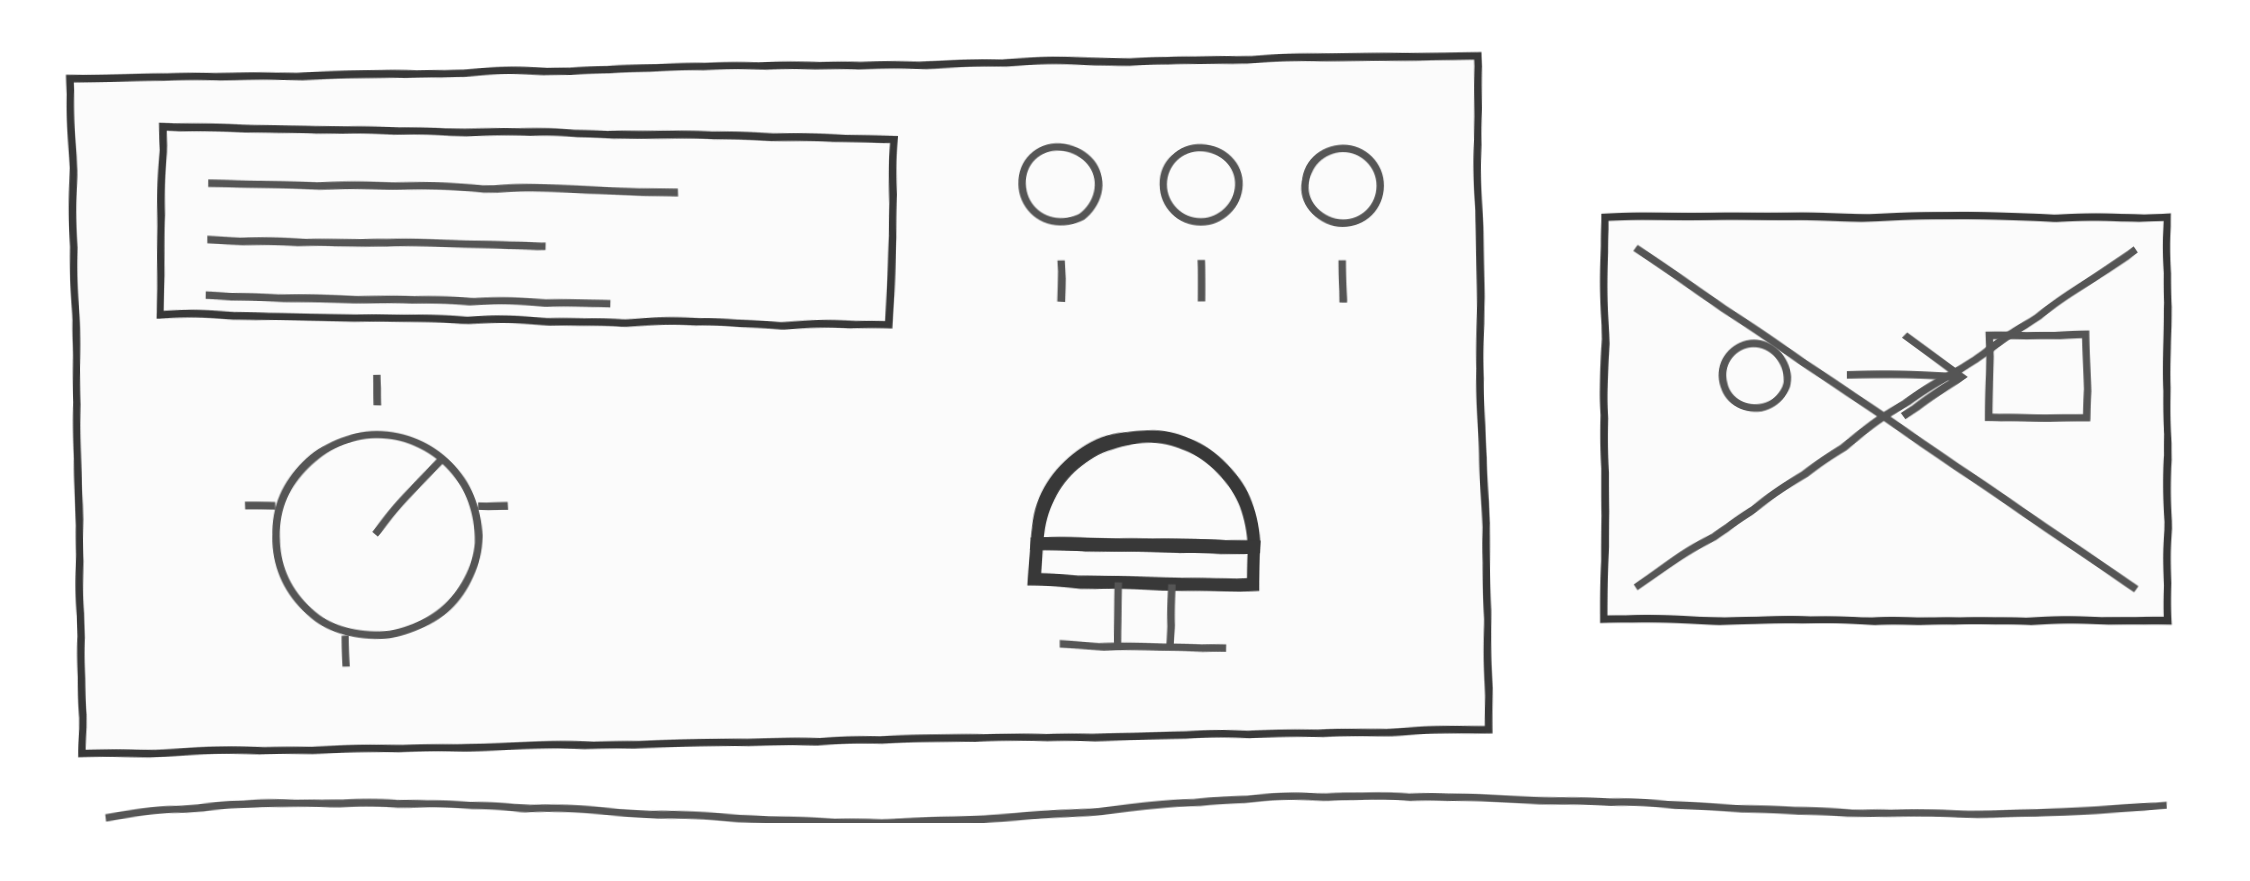
\includegraphics[width=0.96\linewidth,height=0.28\textheight,
 keepaspectratio]{056-operator-panel-pencil.png}

\small\textit{Alternative text: a graphite plate arranges the inert panel this
lesson reasons about: a presentation window of ruled text lines, three status
cells, one detented navigation control, and a heavily drawn mushroom stop
actuator standing apart from the cluster. A crossed-out card to the right holds
a lamp, a drive arrow, and a load block, none of which exist at E0. The plate
is a drawn arrangement for orientation, not a wiring diagram, and no supply,
relay, lamp, or moving part is present.}
\end{center}

\section{Keep the evidence lanes distinct}
\begin{tabularx}{\linewidth}{@{}l X X@{}}
\toprule
Lane & Copied evidence & What it cannot prove\\
\midrule
control & pressed mask, exact source, sequence, time, status & a physical key press\\
stop & asserted level, exact source, sequence, time, status & power removal\\
diagnostic & exact kind and generation & cause recovery by itself\\
presentation & intent generation, observation time, status & visible pixels\\
audit & two complete fixed records & durable storage or atomic writes\\
\bottomrule
\end{tabularx}

Every present aggregate is complete and attributable; every absent aggregate
is canonical zero. A malformed source, invalid mask, stale or ambiguous time,
wrong generation, bad checksum, or structurally inconsistent image rejects
the complete update without partially navigating, clearing a diagnostic,
committing a record, or changing presentation.

\section{Navigate with one qualified control}
The low four mask bits represent \texttt{Previous}, \texttt{Next},
\texttt{Select}, and \texttt{Acknowledge}. Exactly one bit is a valid control.
Zero means no control. A chord, an unknown high bit, a nonadvancing source
sequence, a regressing observation time, or a value older than
\texttt{maximumInputAge} cannot navigate.

\texttt{Previous} and \texttt{Next} wrap within the configured
\texttt{selectableCellCount}. \texttt{Select} requests confirmation;
\texttt{Acknowledge} is not a general-purpose fault eraser. The snapshot keeps
the selected cell, chord disposition, primary diagnostic, audit disposition,
presentation intent, status, and generation independently observable.

\begin{center}
% ADK visual: pencil
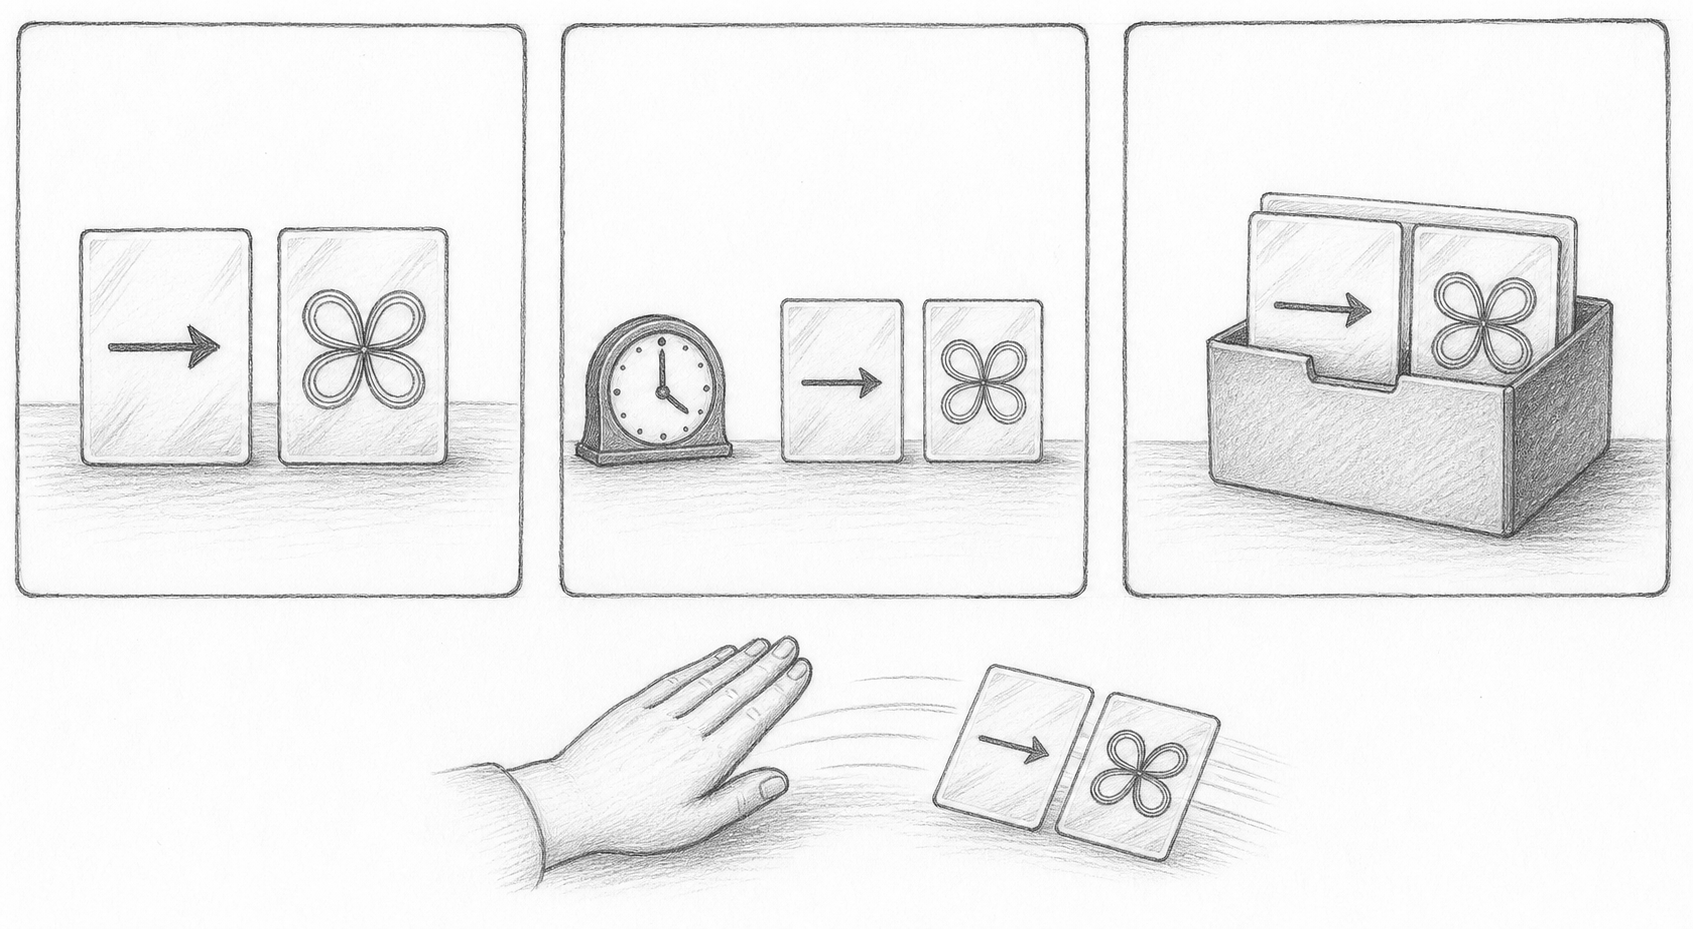
\includegraphics[width=0.96\linewidth,height=0.29\textheight,
 keepaspectratio]{051-joint-preview-pencil.png}

\small\textit{Alternative text: graphite cards show the prepare discipline:
inspect the complete candidate, retain the exact pair until the agreed time,
then place both together; a stopping hand prevents a loose or changed pair
from being applied. In this lesson the pair is a prepared audit record and
its exact acknowledgement.}
\end{center}

\section{Let stop dominate without inventing safety}
An admitted asserted stop dominates control, acknowledgement, presentation
recovery, and a simultaneous solved candidate. It preserves the selected cell,
invalidates live previews, publishes \texttt{Stopped}, and requires a
\texttt{StopAsserted} audit record.

A deasserted level is necessary but not sufficient to release the panel. It
must come from the exact configured source with both a newer modular sequence
and a newer observation time than the retained assertion. The exact
\texttt{StopReleased} record must then commit before the panel leaves stopped
mode. A stale release, a release missing either ordering proof, or an
indeterminate image fails closed.

This is deterministic policy state, not emergency stop. It does not interrupt
power, de-energize a load, detect welded contacts, or establish a safe
electrical state.

\section{Prepare, write, acknowledge, and reconcile}
The caller owns \texttt{PanelAuditImage}, which contains exactly two fixed
slots. The panel copies and validates the complete image; it never retains the
caller's address. An empty image bootstraps sequence one. Later records use the
inactive slot and advance from the unique newest committed predecessor.

\begin{enumerate}
 \item Call \texttt{prepareAudit(operationId, kind, now)}. The returned
       preview binds owner, lifecycle, configuration, epoch, panel generation,
       operation, slot, complete prepared record, and input-image digest.
 \item Copy that prepared record into the named caller-owned slot. This models
       a proposed write; it does not claim physical persistence.
 \item Supply the copied image and exact preview together in one
       \texttt{update}. Complete preflight precedes every mutation.
 \item On success, copy \texttt{canonicalAuditImage()} back to the caller cell.
       The selected record is now committed in the policy image.
\end{enumerate}

Foreign, reconstructed, field-changed, stale, reset-invalidated,
shutdown-invalidated, or consumed previews reject. A prepared record after a
simulated interruption remains visible and requires reconciliation; it is not
silently promoted. Two equally plausible newest records, a sequence gap,
duplicate sequence, invalid state, bad payload digest, or bad checksum is
indeterminate or corrupt and cannot authorize progress.

\section{Acknowledge only exact recoveries}
\texttt{InputRecovered} and \texttt{PresentationRecovered} are the only
acknowledgeable diagnostics. A source or presentation failure first becomes
visible. A later exact healthy observation publishes a recovery diagnostic
with a new generation. \texttt{prepareAcknowledge()} binds that exact live
diagnostic to an exact \texttt{AcknowledgedDiagnostic} audit preview.

The acknowledgement clears only when the update includes the unchanged live
capability and the corresponding prepared audit record. A replacement
diagnostic, asserted stop, reset, shutdown, reconciliation change, wrong
generation, foreign preview, or prior consumption invalidates it. Clue,
configuration, timing, internal, audit, chord, and stopped diagnostics are
never cleared through this route.

\section{Treat presentation as fallible evidence}
\texttt{PanelPresentationIntent} can be \texttt{Blank}, \texttt{Ready},
\texttt{Reviewing}, \texttt{ConfirmationRequired}, \texttt{Solved},
\texttt{Fault}, or \texttt{Stopped}. It binds mode, diagnostic, selected cell,
diagnostic generation, and acknowledgement availability.

Presentation evidence refers to the exact intent generation. A failed
presentation becomes a primary attributable fault. A later exact healthy
observation can publish \texttt{PresentationRecovered}; a stale or mismatched
observation cannot clear anything. Display failure never rewrites the audit
image, releases stop, or changes control provenance.

\section{Run the deterministic replay}
\begin{enumerate}
 \item Initialize. Predict blank intent, released stop, selected cell zero,
       and an unreconciled image. Supply the empty image and observe the
       bootstrap disposition.
 \item Apply one \texttt{Next}. Predict exactly one selected-cell advance.
       Try zero, every valid single bit, each chord, and an unknown high bit.
 \item Inject presentation failure, then its exact healthy recovery. Prepare
       an acknowledgement and retain both preview values.
 \item Collide that acknowledgement with asserted stop, another control, and
       presentation failure. Predict stopped intent, preserved selection, and
       an unusable acknowledgement preview.
 \item Prepare, copy, and acknowledge the exact \texttt{StopAsserted} record.
       Inspect both caller-owned slots and the canonical image.
 \item Try stale, same-sequence, same-time, wrong-source, failed, and
       half-range-ambiguous releases. None may release the panel.
 \item Admit a newer release, then prepare, copy, and acknowledge its exact
       \texttt{StopReleased} record. Predict ready intent only after commit.
 \item Shutdown, initialize, and reconcile a copied image. Replay torn,
       corrupt, duplicate, gap, and two-prepared images without guessing.
\end{enumerate}

\begin{tabularx}{\linewidth}{@{}X X X X X X@{}}
\toprule
time & control & stop & diagnostic & audit state & presentation\\
\midrule
\rule{0pt}{16pt}\blankline & \blankline & \blankline & \blankline & \blankline & \blankline\\[8pt]
\blankline & \blankline & \blankline & \blankline & \blankline & \blankline\\[8pt]
\blankline & \blankline & \blankline & \blankline & \blankline & \blankline\\
\bottomrule
\end{tabularx}

\section{Keep result cells separate}
The Mega replay exposes \texttt{RecoveryCell}, \texttt{CollisionCell},
\texttt{AuditCell}, \texttt{ReleaseCell}, \texttt{RestartCell}, and
\texttt{ReplayCell}. They are the E0 non-Serial observation path.

\begin{tabularx}{\linewidth}{@{}l X X@{}}
\toprule
Cell & Predict and observe & Interpret\\
\midrule
recovery & failure accepted, recovered kind, preview prepared & exact recovery is acknowledgeable\\
collision & stopped, mode, invalidation, preserved selection & stop wins atomically\\
audit & operation, sequence, kind, slot, state, disposition & one exact record committed\\
release & deassert status, audit status, stopped flag, mode & release needs evidence and record\\
restart & initialize, reconcile, stopped, disposition & copied image drives recovery\\
replay & every stage status and final complete bit & one deterministic fixture ran\\
\bottomrule
\end{tabularx}

Compilation does not prove that a powered Mega executed the sketch. On a
powered future display, visible pixels would be separate presentation
evidence; they would not replace these attributed policy cells.

\section{Separate acquisition from safe state}
\textbf{Acquisition prediction and observation.} A valid configuration has
nonzero configuration revision and epoch, a half-range-safe maximum input age,
one to twelve selectable cells, and distinct exact control and stop sources.
Host tests inspect lifecycle generation, copied provenance, immutable
snapshots, previews, images, and result cells.

\textbf{Acquisition interpretation.} Successful initialization proves only
bounded configuration and E0 policy state. It acquires no keypad, stop switch,
display, medium, pin, timer, bus, or registry entry.

\textbf{Safe-state prediction and observation.} Construction, failed
initialization, stop, audit uncertainty, fault, shutdown, and restart publish
blank, fault, or stopped \emph{memory intent} and grant no actuation authority.
This is not proof of a dark indicator, released relay, unlocked exit, or
removed load power.

\section{Read the conservative resource evidence}
The final no-LTO canonical Mega 2560 probe measures 18,118 bytes of flash and
1,454 bytes of static SRAM. The panel object is 365 bytes on AVR; its separate
caller-owned \texttt{PanelAuditImage} is 154 bytes.
Conservative linked-call-graph evidence measures 569 bytes on the deepest
analyzed synchronous stack path.

All four Lesson 056 target gates pass: 24 KiB flash, 2,560 bytes static SRAM,
640 bytes stack, and 384 bytes for the panel object. Residual SRAM is an
aggregate Lesson 057 gate, not a standalone claim here. These are compiler
and link-map results for the exact enhanced fixture, source, flags, Arduino
AVR core 1.8.8, and avr-gcc 7.3.0. They are not runtime high-water
measurements, proof of every interrupt schedule, or physical behavior.

\section{Keep powered work open}
E1 must select and qualify exact passive controls, stop input, display or
indicator, board, supply, electrical endpoints, observation path, pin and
resource map, default and fault states, an authoritative formal schematic,
and recorded bench acceptance. Physical nonvolatile storage is outside this
arc. E2 alone may consider a restrained inert demonstration load with
independent power removal; it can never control access, confinement, egress,
an alarm, or a safety system.

\textbf{Acceptance record.}\quad control/stop provenance: \blankline\quad
recovery collision: \blankline\quad audit sequence: \blankline\\
restart reconciliation: \blankline\quad
acquisition evidence / safe-state evidence: \blankline\ /\ \blankline

Lesson 057 may compose this copied panel state with the Lesson 055 clue model.
It may publish only inert latch, lamp, and presentation intent.

\end{document}
